\begin{frame}{Determining whether two classes are disjoint}
  \begin{columns}[T]
    \begin{column}{0.45\textwidth}
      \usebox\classbox  
    \end{column}%
    \begin{column}{0.55\textwidth}

      \bigskip
      
      \begin{itemize}
      \item<1->{Explicit subtype relation \code{isa?}.}%
      \item<2->{Else if either is \code{:final}; they have no common \Emph{inhabited} subclass.}%
      \item<3->{Else if either is \code{:interface}, there may be class which inherits from both?}%
      \item<4>{If \Emph{currently} no subclass exists, JVM might \Emph{later} run-time
      load \code{subclass.jar} }%
      \end{itemize}
    \end{column}%
  \end{columns}
\end{frame}






\begin{frame}[t]{$MDTD( \{A_1, A_2, \ldots, A_5\})\to\Pi$}
  \scalebox{2.0}{\usebox\boxforestE}
  
  \medskip
  
  Start with $\Sigma=Universe$, and intersect with $A_1$ and $\compl{A_1}$.
\end{frame}



\begin{frame}[t]{$MDTD( \{A_1, A_2, \ldots, A_5\})\to\Pi$}
  \begin{columns}
    \begin{column}{0.6\textwidth}
      \scalebox{1.5}{\usebox\boxforestD}%    
    \end{column}
    \begin{column}{0.4\textwidth}
      {\scalebox{0.7}{\begin{pgfpicture}{0cm}{0cm}{10cm}{6cm} % LL=0,0  UR=10,6
  \pgfcircle[stroke]{\pgfxy(3.5,3)}{3.0cm}   % A   A1
  \pgfputat{\pgfxy(3.5,5.7)}{\pgfbox[center,center]{$A_{1}$}}
  \pgfcircle[stroke]{\pgfxy(2,4)}{1.0cm}   % B    A2
  \pgfputat{\pgfxy(1.5,4.5)}{\pgfbox[center,center]{$A_{2}$}}
  \pgfcircle[stroke]{\pgfxy(3,4.2)}{1.0cm}   % C   A3
  \pgfputat{\pgfxy(3.5,4.6)}{\pgfbox[center,center]{$A_{3}$}}
  \pgfcircle[stroke]{\pgfxy(2.5,2.3)}{1.7cm}   % D A4
  \pgfputat{\pgfxy(1.2,2.7)}{\pgfbox[center,center]{$A_{4}$}}
  \pgfcircle[stroke]{\pgfxy(3.1,1.4)}{0.5cm}   % E   A5
  \pgfputat{\pgfxy(3.2,1.6)}{\pgfbox[center,center]{$A_{5}$}}
  \pgfcircle[stroke]{\pgfxy(5.5,2.0)}{0.5cm}   % F   A6
  \pgfputat{\pgfxy(5.5,2.25)}{\pgfbox[center,center]{$A_{6}$}}
  \pgfcircle[stroke]{\pgfxy(6.7,1.3)}{0.5cm}   % G   A7
  \pgfputat{\pgfxy(6.7,1.5)}{\pgfbox[center,center]{$A_{7}$}}
  \pgfcircle[stroke]{\pgfxy(3.4,1.1)}{1.0cm}   % H   A8
  \pgfputat{\pgfxy(4.0,0.8)}{\pgfbox[center,center]{$A_{8}$}}
\end{pgfpicture}
}}%
    \end{column}
  \end{columns}%
  
  Intersect each leaf with $A_2$ and $\compl{A_2}$.
  \begin{align*}
    A_2 \subset A_1 &\implies A_1\cap A_2 = A_2 & SIMPLIFY\\
    A_2 \subset A_1 &\implies \compl{A_1}\cap A_2 = \emptyset & PRUNE\\
    A_2 \subset A_1 &\implies \compl{A_1}\cap \compl{A_2} = \compl{A_1} & SIMPLIFY
  \end{align*}
\end{frame}

%% \begin{frame}[t]{$MDTD( \{A_1, A_2, \ldots, A_5\})\to\Pi$}
%%   \begin{columns}
%%     \begin{column}{0.6\textwidth}
%%       \scalebox{1.1}{\usebox\boxforestC}
%%     \end{column}
%%     \begin{column}{0.4\textwidth}
%%       {\scalebox{0.7}{\begin{pgfpicture}{0cm}{0cm}{10cm}{6cm} % LL=0,0  UR=10,6
  \pgfcircle[stroke]{\pgfxy(3.5,3)}{3.0cm}   % A   A1
  \pgfputat{\pgfxy(3.5,5.7)}{\pgfbox[center,center]{$A_{1}$}}
  \pgfcircle[stroke]{\pgfxy(2,4)}{1.0cm}   % B    A2
  \pgfputat{\pgfxy(1.5,4.5)}{\pgfbox[center,center]{$A_{2}$}}
  \pgfcircle[stroke]{\pgfxy(3,4.2)}{1.0cm}   % C   A3
  \pgfputat{\pgfxy(3.5,4.6)}{\pgfbox[center,center]{$A_{3}$}}
  \pgfcircle[stroke]{\pgfxy(2.5,2.3)}{1.7cm}   % D A4
  \pgfputat{\pgfxy(1.2,2.7)}{\pgfbox[center,center]{$A_{4}$}}
  \pgfcircle[stroke]{\pgfxy(3.1,1.4)}{0.5cm}   % E   A5
  \pgfputat{\pgfxy(3.2,1.6)}{\pgfbox[center,center]{$A_{5}$}}
  \pgfcircle[stroke]{\pgfxy(5.5,2.0)}{0.5cm}   % F   A6
  \pgfputat{\pgfxy(5.5,2.25)}{\pgfbox[center,center]{$A_{6}$}}
  \pgfcircle[stroke]{\pgfxy(6.7,1.3)}{0.5cm}   % G   A7
  \pgfputat{\pgfxy(6.7,1.5)}{\pgfbox[center,center]{$A_{7}$}}
  \pgfcircle[stroke]{\pgfxy(3.4,1.1)}{1.0cm}   % H   A8
  \pgfputat{\pgfxy(4.0,0.8)}{\pgfbox[center,center]{$A_{8}$}}
\end{pgfpicture}
}}%
%%     \end{column}
%%   \end{columns}%
  
  
%%   \medskip
  
%%   Intersect each leaf with $A_3$ and $\compl{A_3}$.
  
%%   \begin{align*}
%%     A_3 \subset A_1 &\implies \compl{A_1} A_3 = \emptyset & PRUNE
%%   \end{align*}
%% \end{frame}

%% \begin{frame}[t]{$MDTD( \{A_1, A_2, \ldots, A_5\})\to\Pi$}
%%   \scalebox{0.8}{\usebox\boxforestB}
  
%%   \medskip
  
%%   Intersect each leaf with $A_4$ and $\compl{A_4}$.
%% \end{frame}

%% \begin{frame}[t]{$MDTD( \{A_1, A_2, \ldots, A_5\})\to\Pi$}
%%   \scalebox{0.7}{\usebox\boxforestA}
  
%%   \medskip
  
%%   Intersect each leaf with $A_5$ and $\compl{A_5}$.
  
%%   \begin{align*}
%%     A_2 \cap A_5 = \emptyset &\implies A_2A_3A_4A_5 = \emptyset & PRUNE\\
%%     A_5 \subset A_4 &\implies A_1\compl{A_2}~\compl{A_3}~\compl{A_2} \cap A_5=\emptyset & PRUNE\\
%%   \end{align*}
%% \end{frame}

%% \begin{frame}[t]{$MDTD( \{A_1, A_2, \ldots, A_5\})\to\Pi$}
%%   \scalebox{0.7}{\usebox\boxforestA}
  
%%   \medskip
  
%%   Intersect each leaf with $A_5$ and $\compl{A_5}$.
  
%%   \begin{align*}
%%     A_2 \cap A_5 = \emptyset &\implies A_2A_3A_4A_5 = \emptyset & PRUNE\\
%%     A_5 \subset A_4 &\implies A_1\compl{A_2}~\compl{A_3}~\compl{A_2} \cap A_5=\emptyset & PRUNE\\
%%   \end{align*}
%% \end{frame}

\begin{frame}[t]{$MDTD( \{A_1, A_2, \ldots, A_5\})\to\Pi$}
  \scalebox{0.7}{\usebox\boxforestAnu}
  
  \medskip
  
  $MDTD=\Pi \xrightarrow{\leq O(2^n)} \{\typevar_1, \typevar_2, \ldots, \typevar_{10}\} = \{A_2 A_3 A_4,~ A_2 A_3 \compl{A_4}, ~\ldots,~ \compl{A_1}\}$.  
\end{frame}

\begin{frame}[t]{$MDTD( \{A_1, A_2, \ldots, A_5\})\to\Pi$}
  \scalebox{0.65}{\usebox\boxforestAnu}
  
  \medskip
  
  \begin{itemize}
  \item \Emph{By Construction:} either $\typevar_i \subseteq A_j$ or $\typevar_i \subseteq \tynot{A_j}$.
  \item\Emph{By Construction:} $\{\typevar_1, \typevar_2, \ldots, \typevar_{10}\}$ mutually disjoint.
  \item \Emph{By Construction:} $\bigcup_{i=1}^5\typevar_i=\Sigma$.
  \item Exactly the properties we need to compute $\deriv{\typevar}{\singleton{A_i}}$.
  \end{itemize}
\end{frame}




\begin{frame}{Decision Tree Structure}
  We programmatically manipulate \code{if \code{\textcolor{greeny}{then}} ... \code{\textcolor{red}{else}} ...} using a decision tree.

  \begin{columns}
    \begin{column}{0.5\textwidth}
      \includegraphics[height=0.8\textheight]{ldd-0.pdf}
    \end{column}
    \begin{column}{0.5\textwidth}  %%
      \usebox\typecaseAbox
    \end{column}    
  \end{columns}
\end{frame}

\begin{frame}{Decision Tree, Before and After}
  Viewing the decision tree before/after

  \medskip
  
  Rewrite: $1 \to 2\to 3\to 4\to 5\to 6\to 7\to 8\to 9$

  \medskip
  
  \begin{columns}
    \begin{column}{0.5\textwidth}
      \includegraphics[height=0.8\textheight]{ldd-0.pdf}
    \end{column}
    \begin{column}{0.5\textwidth}  %%
      \includegraphics[height=0.8\textheight]{ldd-9.pdf}
    \end{column}
  \end{columns}
\end{frame}


%% Thanks to John Wickerson, https://tex.stackexchange.com/users/25356/john-wickerson
%% for this arrow
%% https://tex.stackexchange.com/questions/113228/how-can-i-add-a-big-arrow
\def\myLeftArrow{\smash{
  \begin{tikzpicture}[baseline=-2mm]
    \useasboundingbox (-2,0);
    \node[single arrow,draw=black,fill=red!10,minimum width=5cm,minimum height=7cm,shape border rotate=180] at (0,-1) {};
  \end{tikzpicture}
}}


\begin{frame}{Rewrite: $\colorbox{orange!30}{\Huge 1}\to 2\to 3\to 4\to 5\to 6\to 7\to 8\to 9$}%1
  Duplicate tree, and introduce \colorbox{pink!30}{\code{if (typep x N) \code{\textcolor{greeny}{then}} ... \code{\textcolor{red}{else}} ...}}

  \begin{columns}
    \begin{column}{0.5\textwidth}
      \only<1,2>{\includegraphics[height=0.8\textheight]{ldd-0.pdf}}%
    \end{column}
    \begin{column}{0.5\textwidth}  %%
      \only<2>{\includegraphics[height=0.8\textheight]{ldd-1.pdf}}%
    \end{column}    
  \end{columns}
\end{frame}

\begin{frame}{Rewrite: $\colorbox{orange!30}{\Huge 1}\to 2\to 3\to 4\to 5\to 6\to 7\to 8\to 9$}%1
  Duplicate tree, and introduce \colorbox{pink!30}{\code{if (typep x N) \code{\textcolor{greeny}{then}} ... \code{\textcolor{red}{else}} ...}}
  
  \centerline{  \includegraphics[height=0.8\textheight]{ldd-1.pdf}}
\end{frame}

\begin{frame}{Rewrite: $1\to \colorbox{orange!30}{\Huge 2}\to 3\to 4\to 5\to 6\to 7\to 8\to 9$}
\begin{tabular}{ll}
  In \code{\textcolor{greeny}{then}}: \colorbox{pink!30}{Supertypes of \code{N} $\to$ \code{:sigma}}. &
  In \code{\textcolor{red}{else}}: \colorbox{pink!30}{Subtypes of \code{N} $\to$ \code{:empty-set}}.
  \end{tabular}
  
  \only<1>{\centerline{\includegraphics[height=0.8\textheight]{ldd-1.pdf}}}%
  \only<2>{\centerline{\includegraphics[height=0.8\textheight]{ldd-2.pdf}}}
\end{frame}

\begin{frame}{Rewrite: $1\to 2\to \colorbox{orange!30}{\Huge 3}\to 4\to 5\to 6\to 7\to 8\to 9$}
  \begin{tabular}{ll}
    \colorbox{pink!30}{\code{(not :sigma)} $\to$ \code{:empty-set}} &       \colorbox{pink!30}{\code{(not :empty-set)} $\to$ \code{:sigma}}    
  \end{tabular}

  \only<1>{\centerline{\includegraphics[height=0.8\textheight]{ldd-2.pdf}}}%
  \only<2>{\centerline{\includegraphics[height=0.8\textheight]{ldd-3.pdf}}}
\end{frame}

\begin{frame}{Rewrite: $1\to 2\to 3\to \colorbox{orange!30}{\Huge 4}\to 5\to 6\to 7\to 8\to 9$}
  \begin{tabular}{ll}
    \colorbox{pink!30}{\code{(:sigma \& x)} $\to$ \code{x}} &       \colorbox{pink!30}{\code{(:empty-set \& x)} $\to$ \code{:empty-set}}
  \end{tabular}
  \only<1>{\centerline{\includegraphics[height=0.8\textheight]{ldd-3.pdf}}}%
  \only<2>{\centerline{\includegraphics[height=0.8\textheight]{ldd-4.pdf}}}
\end{frame}


\begin{frame}{Rewrite: $1\to 2\to 3\to 4\to\colorbox{orange!30}{\Huge 5}\to 6\to 7\to 8\to 9$}
  \begin{tabular}{ll}
    Replace \usebox\boxstop~with \code{\textcolor{greeny}{then}} branch. &
    Replace \usebox\boxsempty~with \code{\textcolor{red}{else}} branch.
  \end{tabular}

  \only<1>{\centerline{\includegraphics[height=0.8\textheight]{ldd-4.pdf}}}%
  \only<2>{\centerline{\includegraphics[height=0.8\textheight]{ldd-5.pdf}}}
  
\end{frame}


\begin{frame}{Rewrite: $1\to 2\to 3\to 4\to 5\to \colorbox{orange!30}{\Huge 6}\to 7\to 8\to 9$}
  Duplicate tree, and introduce \colorbox{pink!30}{\code{if (typep x I) \code{\textcolor{greeny}{then}} ... \code{\textcolor{red}{else}} ...}}

  \begin{columns}
    \begin{column}{0.5\textwidth}
      \includegraphics[height=0.8\textheight]{ldd-5.pdf}%
    \end{column}

    \begin{column}{0.5\textwidth}  %%
      \includegraphics[height=0.8\textheight]{ldd-6.pdf}%
    \end{column}    
  \end{columns}
\end{frame}

\begin{frame}{Rewrite: $1\to 2\to 3\to 4\to 5\to \colorbox{orange!30}{\Huge 6}\to 7\to 8\to 9$}
  Duplicate tree, and introduce \colorbox{pink!30}{\code{if (typep x I) \code{\textcolor{greeny}{then}} ... \code{\textcolor{red}{else}} ...}}

  \centerline{\includegraphics[height=0.8\textheight]{ldd-6.pdf}}  %
\end{frame}


\begin{frame}{Rewrite: $1\to 2\to 3\to 4\to 5\to 6\to \colorbox{orange!30}{\Huge 7}\to 8\to 9$}
  \begin{tabular}{ll}
  In \code{\textcolor{greeny}{then}}: \colorbox{pink!30}{Supertypes of \code{I} $\to$ \code{:sigma}}.&
  In \code{\textcolor{red}{else}}: \colorbox{pink!30}{Subtypes of \code{I} $\to$ \code{:empty-set}}.
  \end{tabular}

  \only<1>{\centerline{\includegraphics[height=0.8\textheight]{ldd-6.pdf}}}%
  \only<2>{\centerline{\includegraphics[height=0.8\textheight]{ldd-7.pdf}}}
\end{frame}


\begin{frame}{Rewrite: $1\to 2\to 3\to 4\to 5\to 6\to 7\to \colorbox{orange!30}{\Huge 8}\to 9$}
  \begin{tabular}{ll}
      \colorbox{pink!30}{\code{(not :sigma)} $\to$ \code{:empty-set}} &    
      \colorbox{pink!30}{\code{(not :empty-set)} $\to$ \code{:sigma}}
  \end{tabular}

  \only<1>{\centerline{\includegraphics[height=0.8\textheight]{ldd-7.pdf}}}%
  \only<2>{\centerline{\includegraphics[height=0.8\textheight]{ldd-8.pdf}}}
\end{frame}

\begin{frame}{Rewrite: $1\to 2\to 3\to 4\to 5\to 6\to 7\to 8\to \colorbox{orange!30}{\Huge 9}$}
  \begin{tabular}{ll}
    Replace \usebox\boxstop~ with \code{\textcolor{greeny}{then}} branch. &
    Replace \usebox\boxsempty~ with \code{\textcolor{red}{else}} branch.
  \end{tabular}

  \only<1>{\centerline{\includegraphics[height=0.8\textheight]{ldd-8.pdf}}}%
  \only<2>{\centerline{\includegraphics[height=0.8\textheight]{ldd-9.pdf}}}
  

\end{frame}


\begin{frame}{Rewrite: Summary}
  Code has been rewritten so that \Emph{any type check occurs no more than once}.

  \begin{columns}
    \begin{column}{0.5\textwidth}
      \usebox\typecaseAbox
    \end{column}
    \begin{column}{0.5\textwidth}  %%
      \usebox\typecaseKbox
    \end{column}
  \end{columns}

  And it is clear the code never returns \code{nil}.

\end{frame}




%% --------------------


\begin{frame}{Setup}{Declaration Clojure Code}
  \begin{columns}
    \begin{column}{0.5\textwidth}
      \usebox\demoBbox
    \end{column}
    \begin{column}{0.5\textwidth}
      \only<1>{\usebox\demoAbox}%
      \only<2>{\usebox\demoCbox}%
    \end{column}
  \end{columns}
\end{frame}


\begin{frame}{DFAs}
  \only<1>{\usebox\demoDbox}%
  \only<2>{\usebox\demoEbox}%
  \only<3>{\usebox\demoFbox}%

  \only<1>{\Large
    \begin{align*}
      t_0 &= \text{\code{String}}\\
      t_1 &= \text{\code{(or String (? even))}}
    \end{align*}}%
  \only<2>{\Large
    \begin{align*}
      t_0 &= \text{\code{String}}\\
      t_1 &= \text{\code{(or String (and Integer (? even)))}}
    \end{align*}}%
  \only<3>{\Large
    \begin{align*}
      t_0 &= \text{\code{String}}\\
      t_1 &= \text{\code{(or String (and Integer (? even) (? large)))}}
    \end{align*}}

  \only<1>{\centering\includegraphics[width=8cm]{pat1}}%
  \only<2>{\centering\includegraphics[width=8cm]{pat2}}%
  \only<3>{\centering\includegraphics[width=8cm]{pat3}}%
\end{frame}

\begin{frame}{Inclusion Checks}
  \usebox\demoGbox

  By inspection we see that \[\sem{pat3} \subsetneq \sem{pat2} = \sem{pat1}\,.\]
  Can we determine this programmatically?
\end{frame}



\begin{frame}{Inclusion Checks}

  \only<1>{\[\sem{pat3} \subsetneq \underbrace{\sem{pat2} = \sem{pat1}}_{\sem{pat2}~ \subset~ \sem{pat1}~ =~ YES}\]}%
  \only<2>{\[\sem{pat3} \subsetneq \underbrace{\sem{pat2} = \sem{pat1}}_{\sem{pat2}~ \supset~ \sem{pat1}~ =~ DONT-KNOW}\]}%
  \only<3>{\[\underbrace{\sem{pat3} \subsetneq \sem{pat2}}_{YES} = \sem{pat1}\]}%
  \only<4>{\[\sem{pat2} \cap \overline{\sem{pat3}}\]}%

  \begin{columns}
    \begin{column}{0.5\textwidth}
      \only<1>{\usebox\demoHbox}%
      \only<2>{\usebox\demoIbox}%
      \only<3>{\usebox\demoJbox}%
      \only<4>{\usebox\demoKbox}%
    \end{column}
    \begin{column}{0.5\textwidth}
      \only<1>{
        \begin{align*}
          t_0 &= \text{\code{String}}\\
          t_1 &= \text{\code{(or String (and Integer (? even)))}}
        \end{align*}
        %                          [trim={left bottom right top},clip]
        \includegraphics[width=8cm,trim={0 0 0 15mm},clip]{p2-p1}
      }%
      \only<2>{
    \begin{align*}
      t_0 &= \text{\code{S}}\\
      t_1 &= \text{\code{!I \& !S \& Even}} && Indeterminate\\
      t_2 &= \text{\code{S | (I \& Even)}}\\
      t_3 &= \text{\code{S | Even}}
    \end{align*}
    %                          [trim={left bottom right top},clip]
    \includegraphics[width=8cm,trim={0 0 0 15mm},clip]{p1-p2}
      }%
      \only<3>{
    \begin{align*}
      t_0 &= \text{\code{S}}\\
      t_1 &= \text{\code{S | (I \& Even, Large)}}
    \end{align*}
    %                          [trim={left bottom right top},clip]
    \includegraphics[width=8cm,trim={0 0 0 15mm},clip]{p3-p2}
      }%
      \only<4>{
        \begin{align*}
          t_0 &= \text{\code{S}}\\
          t_1 &= \text{\code{I \& Even \& !Large}}\\
          t_2 &= \text{\code{S | (I \& Even \& Large)}}\\
          t_3 &= \text{\code{S | (I \& Even)}}\\
        \end{align*}
        %                          [trim={left bottom right top},clip]
        \includegraphics[width=8cm,trim={0 0 0 15mm},clip]{p2-p3}
      }
    \end{column}
  \end{columns}
\end{frame}

%\subsection{Vacuity: Habitation Checks}

{  %% chapter slide
  \setbeamercolor{background canvas}{bg=sectioncolor}
\begin{frame}{\Challenge{6} How to detect habitation/vacuity in a DFA}

  \centering
  \includegraphics[width=\linewidth]{p4-p3}
\end{frame}
}

\newsavebox\demoAbox
\begin{lrbox}{\demoAbox}
  \begin{minipage}{8cm}
    %% dont re-indent this file
\begin{lstlisting}[style=reclojureScala]
def large(n:Any):Boolean = {
  n match {
    case n: Int => n > 127
    case _ => false
  }
}

def even(n:Any):Boolean = {
  n match {
    case n: Int => n % 2 == 0
    case _ => false
  }
}
\end{lstlisting}

  \end{minipage}
\end{lrbox}

\newsavebox\demoBbox
\begin{lrbox}{\demoBbox}
  \begin{minipage}{8cm}
    %% dont re-indent this file
\begin{lstlisting}[style=reclojureClojure]
(def pat-1
  '(:* (:cat String
             (:* (? even)))))
(def pat-2
  '(:* (:cat String
             (:* (and Integer 
                      (? even))))))
(def pat-3
  '(:* (:cat String
             (:* (and Integer
                      (? even)
                      (? large))))))
\end{lstlisting}

  \end{minipage}
\end{lrbox}

\newsavebox\demoCbox
\begin{lrbox}{\demoCbox}
  \begin{minipage}{8cm}
    %% dont re-indent this file
\begin{lstlisting}[style=reclojureScala]
val data:Seq[Any] = 
  Seq("Lorem",
      "ipsum", 2, 4, 8,
      "dolor", 10, 20)

pat1.contains(data)
// --> true

pat2.contains(data)
// --> true

pat3.contains(data)
// --> false
\end{lstlisting}

  \end{minipage}
\end{lrbox}



\begin{frame}{Setup}{Declaration Scala Code}
  \begin{columns}
    \begin{column}{0.5\textwidth}
      \usebox\demoBbox
    \end{column}
    \begin{column}{0.5\textwidth}
      \only<1>{\usebox\demoAbox}%
      \only<2>{\usebox\demoCbox}%
    \end{column}
  \end{columns}
\end{frame}

\newsavebox\demoDbox
\begin{lrbox}{\demoDbox}
  \begin{minipage}{16cm}
    %% dont re-indent this file
\begin{lstlisting}[style=reclojureScala]
pat1 = (S ++ Even.*).*
dfaView(pat1.toDfa())
\end{lstlisting}

  \end{minipage}
\end{lrbox}
\newsavebox\demoEbox
\begin{lrbox}{\demoEbox}
  \begin{minipage}{16cm}
    %% dont re-indent this file
\begin{lstlisting}[style=reclojureClojure]
(let [pat-2 '(:* (:cat String (:* (and Integer (? even)))))]
  (dfa-to-dot pat-2 :view true))
\end{lstlisting}

  \end{minipage}
\end{lrbox}
\newsavebox\demoFbox
\begin{lrbox}{\demoFbox}
  \begin{minipage}{16cm}
    %% dont re-indent this file
\begin{lstlisting}[style=reclojureScala]
pat3 = (S ++ (I & Even & Large).*).*
dfaView(pat3.toDfa())
\end{lstlisting}

  \end{minipage}
\end{lrbox}
\newsavebox\demoGbox
\begin{lrbox}{\demoGbox}
  \begin{minipage}{16cm}
    %% dont re-indent this file
\begin{lstlisting}[style=reclojureScala]
val pat1 = (S ++ Even.*).*
val pat2 = (S ++ (I & Even).*).*
val pat3 = (S ++ (I & Even & Large).*).*
\end{lstlisting}

  \end{minipage}
\end{lrbox}

\newsavebox\demoHbox
\begin{lrbox}{\demoHbox}
  \begin{minipage}{8cm}
    %% dont re-indent this file
\begin{lstlisting}[style=reclojureClojure]
(let [pat-1 '(:* (:cat String (? even)))
      pat-2 '(:* (:cat String (and Integer
                                   (? even))))
      diff-21 (gns/- pat-2 pat-1)]

 ;; emptyset if pat2 subset of pat1
 (dfa-to-dot diff-21 :view true))
\end{lstlisting}

  \end{minipage}
\end{lrbox}


\newsavebox\demoIbox
\begin{lrbox}{\demoIbox}
  \begin{minipage}{8cm}
    %% dont re-indent this file
\begin{lstlisting}[style=reclojureScala]
val pat1 = (S ++ Even.*).*
val pat2 = (S ++ (I & Even).*).*
val pat3 = (S ++ (I & Even & Large).*).*

// emptyset if pat1 subset of pat2
val diff12 = pat1 - pat2
dfaView(diff12.toDfa())
\end{lstlisting}

  \end{minipage}
\end{lrbox}

\newsavebox\demoJbox
\begin{lrbox}{\demoJbox}
  \begin{minipage}{8cm}
    %% dont re-indent this file
\begin{lstlisting}[style=reclojureClojure]
(let [pat-1 '(:* String (:* (? even)))
      pat-2 '(:* (:cat String (and Integer (? even))))
      pat-3 '(:* (:cat String (and Integer
                                   (? even) 
                                   (? large))))
      diff-32 (template (and ~pat-3 (not ~pat-2)))]

  ;; emptyset if pat3 subset of pat2
  (dfa-to-dot diff-32 :view true))
\end{lstlisting}

  \end{minipage}
\end{lrbox}

\newsavebox\demoKbox
\begin{lrbox}{\demoKbox}
  \begin{minipage}{8cm}
    %% dont re-indent this file
\begin{lstlisting}[style=reclojureClojure]
(let [pat-1 '(:* (:cat String (:* (? even))))
      pat-2 '(:* (:cat String (:* (and Long (? even)))))
      pat-3 '(:* (:cat String (:* (and Long (? even) (? large)))))
      diff-23 (gns/- pat-2 pat-3)]

   ;; Example of element in pat2 but not pat3
   (dfa-to-dot diff-23 :view true))
\end{lstlisting}

  \end{minipage}
\end{lrbox}




\begin{frame}{DFAs}
  \only<1>{\usebox\demoDbox}%
  \only<2>{\usebox\demoEbox}%
  \only<3>{\usebox\demoFbox}%

  \only<1>{\Large
    \begin{align*}
      t_0 &= \text{\code{String}}\\
      t_1 &= \text{\code{(or String (? even))}}
    \end{align*}}%
  \only<2>{\Large
    \begin{align*}
      t_0 &= \text{\code{String}}\\
      t_1 &= \text{\code{(or String (and Integer (? even)))}}
    \end{align*}}%
  \only<3>{\Large
    \begin{align*}
      t_0 &= \text{\code{String}}\\
      t_1 &= \text{\code{(or String (and Integer (? even) (? large)))}}
    \end{align*}}

  \only<1>{\centering\includegraphics[width=8cm]{pat1}}%
  \only<2>{\centering\includegraphics[width=8cm]{pat2}}%
  \only<3>{\centering\includegraphics[width=8cm]{pat3}}%
\end{frame}

\begin{frame}{Inclusion Checks}
  \usebox\demoGbox

  By inspection we see that \[\sem{pat3} \subsetneq \sem{pat2} = \sem{pat1}\,.\]
  Can we determine this programmatically?
\end{frame}



\begin{frame}{Inclusion Checks}

  \only<1>{\[\sem{pat3} \subsetneq \underbrace{\sem{pat2} = \sem{pat1}}_{\sem{pat2}~ \subset~ \sem{pat1}~ =~ YES}\]}%
  \only<2>{\[\sem{pat3} \subsetneq \underbrace{\sem{pat2} = \sem{pat1}}_{\sem{pat2}~ \supset~ \sem{pat1}~ =~ DONT-KNOW}\]}%
  \only<3>{\[\underbrace{\sem{pat3} \subsetneq \sem{pat2}}_{YES} = \sem{pat1}\]}%
  \only<4>{\[\sem{pat2} \cap \overline{\sem{pat3}}\]}%

  \begin{columns}
    \begin{column}{0.5\textwidth}
      \only<1>{\usebox\demoHbox}%
      \only<2>{\usebox\demoIbox}%
      \only<3>{\usebox\demoJbox}%
      \only<4>{\usebox\demoKbox}%
    \end{column}
    \begin{column}{0.5\textwidth}
      \only<1>{
        \begin{align*}
          t_0 &= \text{\code{String}}\\
          t_1 &= \text{\code{(or String (and Integer (? even)))}}
        \end{align*}
        %                          [trim={left bottom right top},clip]
        \includegraphics[width=8cm,trim={0 0 0 15mm},clip]{p2-p1}
      }%
      \only<2>{
    \begin{align*}
      t_0 &= \text{\code{S}}\\
      t_1 &= \text{\code{!I \& !S \& Even}} && Indeterminate\\
      t_2 &= \text{\code{S | (I \& Even)}}\\
      t_3 &= \text{\code{S | Even}}
    \end{align*}
    %                          [trim={left bottom right top},clip]
    \includegraphics[width=8cm,trim={0 0 0 15mm},clip]{p1-p2}
      }%
      \only<3>{
    \begin{align*}
      t_0 &= \text{\code{S}}\\
      t_1 &= \text{\code{S | (I \& Even, Large)}}
    \end{align*}
    %                          [trim={left bottom right top},clip]
    \includegraphics[width=8cm,trim={0 0 0 15mm},clip]{p3-p2}
      }%
      \only<4>{
        \begin{align*}
          t_0 &= \text{\code{S}}\\
          t_1 &= \text{\code{I \& Even \& !Large}}\\
          t_2 &= \text{\code{S | (I \& Even \& Large)}}\\
          t_3 &= \text{\code{S | (I \& Even)}}\\
        \end{align*}
        %                          [trim={left bottom right top},clip]
        \includegraphics[width=8cm,trim={0 0 0 15mm},clip]{p2-p3}
      }
    \end{column}
  \end{columns}
\end{frame}


\begin{frame}{Habitation Check}

  Is the language of the DFA inhabited?
  \begin{itemize}
  \item YES -- satisfiable path to accepting state
  \item NO -- no path to accepting state
  \item DONT-KNOW -- only indeterminate paths to accepting state
  \end{itemize}

  \includegraphics[width=\linewidth]{p4-p3}

\end{frame}


\begin{frame}{Habitation Check}

  How do Dijkstra weights work?

  \only<1>{\scalebox{0.8}{\documentclass{standalone}
  \usepackage{tikz}
  \usetikzlibrary{arrows.meta, automata, bending, positioning, shapes.misc}
  \tikzstyle{automaton}=[shorten >=1pt, >={Stealth[bend,round]}, initial text=]
  \tikzstyle{accepting}=[double]

\begin{document}
\begin{tikzpicture}[automaton, auto, thick]
  \node[state,initial,rounded rectangle] (0) {$0$};
  \node[state,color=red,rounded rectangle] (1) [above right=7mm and 50mm of 0] {$1$};
  \node[state,text=black,accepting,rounded rectangle] (2) [right=50mm of 1] {$2$};
  \node[state,text=black,rounded rectangle] (3) [below right=7mm and 35mm of 0] {$3$};
  \node[state,text=black,rounded rectangle] (4) [right=35mm of 3] {$4$};
  \path[->] (0) edge[color=indeterminate, dotted, line width=3pt] node {$Int \cap Odd$} (1);
  \path[->] (0) edge[swap] node {$\overline{Int}$} (3);
  \path[->] (1) edge[color=indeterminate, dotted, line width=3pt]  node[pos=.5] {$Int$} (2);
  \path[->] (3) edge    node {$String$} (4);
  \path[->] (4) edge[swap]    node {$Float$} (2);
\end{tikzpicture}
\end{document}
}}%
  \only<2,3>{\scalebox{0.8}{\documentclass{standalone}
  \usepackage{tikz}
  \usetikzlibrary{arrows.meta, automata, bending, positioning, shapes.misc}
  \tikzstyle{automaton}=[shorten >=1pt, >={Stealth[bend,round]}, initial text=]
  \tikzstyle{accepting}=[double]

\begin{document}
\begin{tikzpicture}[automaton, auto, thick]
  \node[state,initial,rounded rectangle] (0) {$0$};
  \node[state,color=red,rounded rectangle] (1) [above right=7mm and 50mm of 0] {$1$};
  \node[state,text=black,accepting,rounded rectangle] (2) [right=50mm of 1] {$2$};
  \node[state,text=black,rounded rectangle] (3) [below right=7mm and 35mm of 0] {$3$};
  \node[state,text=black,rounded rectangle] (4) [right=35mm of 3] {$4$};
  \path[->] (0) edge[color=indeterminate, dotted, line width=3pt] node {$Int \cap Odd$} (1);
  \path[->] (0) edge[swap] node {$\overline{Int} ~ \textcolor{blue}{[W\!\!=\!1]}$} (3);
  \path[->] (1) edge[color=indeterminate, dotted, line width=3pt]  node[pos=.5] {$Int$ \textcolor{blue}{$[W\!\!=\!1]$}} (2);
  \path[->] (3) edge    node {$String ~ \textcolor{blue}{[W\!\!=\!1]}$} (4);
  \path[->] (4) edge[swap]    node {$Float ~ \textcolor{blue}{[W\!\!=\!1]}$} (2);
\end{tikzpicture}
\end{document}
}}%
  \only<4->{\scalebox{0.8}{\documentclass{standalone}
  \usepackage{tikz}
  \usetikzlibrary{arrows.meta, automata, bending, positioning, shapes.misc}
  \tikzstyle{automaton}=[shorten >=1pt, >={Stealth[bend,round]}, initial text=]
  \tikzstyle{accepting}=[double]

\begin{document}
\begin{tikzpicture}[automaton, auto, thick]
  \node[state,initial,rounded rectangle] (0) {$0$};
  \node[state,color=red,rounded rectangle] (1) [above right=7mm and 50mm of 0] {$1$};
  \node[state,text=black,accepting,rounded rectangle] (2) [right=50mm of 1] {$2$};
  \node[state,text=black,rounded rectangle] (3) [below right=7mm and 35mm of 0] {$3$};
  \node[state,text=black,rounded rectangle] (4) [right=35mm of 3] {$4$};
  \path[->] (0) edge[color=indeterminate, dotted, line width=3pt] node {$Int \cap Odd  ~ \textcolor{red}{[W\!\!=\!5]}$} (1);
  \path[->] (0) edge[swap] node {$\overline{Int} ~ \textcolor{blue}{[W\!\!=\!1]}$} (3);
  \path[->] (1) edge[color=indeterminate, dotted, line width=3pt]  node[pos=.5] {$Int$ \textcolor{blue}{$[W\!\!=\!1]$}} (2);
  \path[->] (3) edge    node {$String ~ \textcolor{blue}{[W\!\!=\!1]}$} (4);
  \path[->] (4) edge[swap]    node {$Float ~ \textcolor{blue}{[W\!\!=\!1]}$} (2);
\end{tikzpicture}
\end{document}
}}%

  \begin{itemize}
  \item<2->{Satisfiable transitions have weight \textcolor{blue}{$W\!=1$}.}
  \item<3->{Unsatisfiable transitions have weight \textcolor{red}{$W\!=\infty$}.}
  \item<4->{Indeterminate transitions have weight \textcolor{red}{$W\!=5$} (number of states).}
  \item<5>{Shortest path is $\nodecirc{0} \xrightarrow{1} \nodecirc{3} \xrightarrow{1} \nodecirc{4}  \xrightarrow{1} \nodecirc{2}$; length is $3$\\
  Longer path is $\nodecirc{0}\xrightarrow{5}\nodecirc{1}\xrightarrow{1}\nodecirc{2}$; length is $6$}
  \end{itemize}
\end{frame}





\begin{frame}{Habitation Check}

  How do Dijkstra weights work?

  \only<1>{\scalebox{0.8}{\documentclass{standalone}
  \usepackage{tikz}
  \usetikzlibrary{arrows.meta, automata, bending, positioning, shapes.misc}
  \tikzstyle{automaton}=[shorten >=1pt, >={Stealth[bend,round]}, initial text=]
  \tikzstyle{accepting}=[double]

\begin{document}
\begin{tikzpicture}[automaton, auto, thick]
  \node[state,initial,rounded rectangle] (0) {$0$};
  \node[state,color=red,rounded rectangle] (1) [above right=7mm and 50mm of 0] {$1$};
  \node[state,text=black,accepting,rounded rectangle] (2) [right=50mm of 1] {$2$};
  \node[state,text=black,rounded rectangle] (3) [below right=7mm and 35mm of 0] {$3$};
  \node[state,text=black,rounded rectangle] (4) [right=35mm of 3] {$4$};
  \path[->] (0) edge[color=indeterminate, dotted, line width=3pt] node {$Int \cap Odd$} (1);
  \path[->] (0) edge[swap] node {$\overline{Int}$} (3);
  \path[->] (1) edge[color=indeterminate, dotted, line width=3pt]  node[pos=.5] {$Int$} (2);
  \path[->] (3) edge    node {$String$} (4);
  \path[->] (4) edge[swap]    node {$Float$} (2);
\end{tikzpicture}
\end{document}
}}%
  \only<2,3>{\scalebox{0.8}{\documentclass{standalone}
  \usepackage{tikz}
  \usetikzlibrary{arrows.meta, automata, bending, positioning, shapes.misc}
  \tikzstyle{automaton}=[shorten >=1pt, >={Stealth[bend,round]}, initial text=]
  \tikzstyle{accepting}=[double]

\begin{document}
\begin{tikzpicture}[automaton, auto, thick]
  \node[state,initial,rounded rectangle] (0) {$0$};
  \node[state,color=red,rounded rectangle] (1) [above right=7mm and 50mm of 0] {$1$};
  \node[state,text=black,accepting,rounded rectangle] (2) [right=50mm of 1] {$2$};
  \node[state,text=black,rounded rectangle] (3) [below right=7mm and 35mm of 0] {$3$};
  \node[state,text=black,rounded rectangle] (4) [right=35mm of 3] {$4$};
  \path[->] (0) edge[color=indeterminate, dotted, line width=3pt] node {$Int \cap Odd$} (1);
  \path[->] (0) edge[swap] node {$\overline{Int} ~ \textcolor{blue}{[W\!\!=\!1]}$} (3);
  \path[->] (1) edge[color=indeterminate, dotted, line width=3pt]  node[pos=.5] {$Int$ \textcolor{blue}{$[W\!\!=\!1]$}} (2);
  \path[->] (3) edge    node {$String ~ \textcolor{blue}{[W\!\!=\!1]}$} (4);
  \path[->] (4) edge[swap]    node {$Float ~ \textcolor{blue}{[W\!\!=\!1]}$} (2);
\end{tikzpicture}
\end{document}
}}%
  \only<4->{\scalebox{0.8}{\documentclass{standalone}
  \usepackage{tikz}
  \usetikzlibrary{arrows.meta, automata, bending, positioning, shapes.misc}
  \tikzstyle{automaton}=[shorten >=1pt, >={Stealth[bend,round]}, initial text=]
  \tikzstyle{accepting}=[double]

\begin{document}
\begin{tikzpicture}[automaton, auto, thick]
  \node[state,initial,rounded rectangle] (0) {$0$};
  \node[state,color=red,rounded rectangle] (1) [above right=7mm and 50mm of 0] {$1$};
  \node[state,text=black,accepting,rounded rectangle] (2) [right=50mm of 1] {$2$};
  \node[state,text=black,rounded rectangle] (3) [below right=7mm and 35mm of 0] {$3$};
  \node[state,text=black,rounded rectangle] (4) [right=35mm of 3] {$4$};
  \path[->] (0) edge[color=indeterminate, dotted, line width=3pt] node {$Int \cap Odd  ~ \textcolor{red}{[W\!\!=\!5]}$} (1);
  \path[->] (0) edge[swap] node {$\overline{Int} ~ \textcolor{blue}{[W\!\!=\!1]}$} (3);
  \path[->] (1) edge[color=indeterminate, dotted, line width=3pt]  node[pos=.5] {$Int$ \textcolor{blue}{$[W\!\!=\!1]$}} (2);
  \path[->] (3) edge    node {$String ~ \textcolor{blue}{[W\!\!=\!1]}$} (4);
  \path[->] (4) edge[swap]    node {$Float ~ \textcolor{blue}{[W\!\!=\!1]}$} (2);
\end{tikzpicture}
\end{document}
}}%

  \begin{itemize}
  \item<2->{Satisfiable transitions have weight \textcolor{blue}{$W\!=1$}.}
  \item<3->{Unsatisfiable transitions have weight \textcolor{red}{$W\!=\infty$}.}
  \item<4->{Indeterminate transitions have weight \textcolor{red}{$W\!=5$} (number of states).}
  \item<5>{Shortest path is $\nodecirc{0} \xrightarrow{1} \nodecirc{3} \xrightarrow{1} \nodecirc{4}  \xrightarrow{1} \nodecirc{2}$; length is $3$\\
  Longer path is $\nodecirc{0}\xrightarrow{5}\nodecirc{1}\xrightarrow{1}\nodecirc{2}$; length is $6$}
  \end{itemize}
\end{frame}



%\subsection{Efficiency: Redundant Type Checks}

{  %% chapter slide
  \setbeamercolor{background canvas}{bg=sectioncolor}

\begin{frame}{\Challenge{5} Redundant Type Check}
  Select correct transition, avoiding \Emph{redundant type checks}.

  \medskip

  \scalebox{0.85}{\documentclass{standalone}
  \usepackage{tikz}
  \usetikzlibrary{arrows.meta, automata, bending, positioning, shapes.misc}
  \tikzstyle{automaton}=[shorten >=1pt, >={Stealth[bend,round]}, initial text=]

\begin{document}
\begin{tikzpicture}[automaton, auto, thick]
  \node[state,initial,rounded rectangle] (0) {$0$};
  \node[state,accepting,thick,rounded rectangle] (2) [right=30mm of 0] {$2$};
  \node[state,accepting,thick,rounded rectangle] (1) [above right=7mm and 30mm of 0] {$1$};
  \node[state,accepting,thick,rounded rectangle] (3) [below right=7mm and 30mm of 0] {$3$};
  \path[->] (0) edge node {$Int$} (2);
  \path[->] (0) edge[bend left=15]  node[pos=.8] {$Number~ \cap~ !Int$} (1);
  \path[->] (0) edge[bend right=15] node[swap] {$!~Number$} (3);
\end{tikzpicture}
\end{document}
}
\end{frame}
}


\newsavebox\typecaseAbox
\begin{lrbox}{\typecaseAbox}
  \begin{minipage}{8cm}
    %% dont re-indent this file
\begin{lstlisting}[style=reclojureClojure]
(typecase x
  (and Number (not Long))
  1

  Long
  2

  (not Number)
  3)
\end{lstlisting}

  \end{minipage}
\end{lrbox}

\newsavebox\typecaseITEbox
\begin{lrbox}{\typecaseITEbox}
  \begin{minipage}{8cm}
    %% dont re-indent this file
\begin{lstlisting}[style=reclojureScala]
Ite(N & !I, Some(1),
            Ite(I, Some(2),
                    Ite(!N, Some(3),
                           None)))
\end{lstlisting}

  \end{minipage}
\end{lrbox}

\newsavebox\typecaseITEafterbox
\begin{lrbox}{\typecaseITEafterbox}
  \begin{minipage}{8cm}
%% dont re-indent this file
\begin{lstlisting}[style=reclojureScala]
Ite(N, Ite(I, Some(2),
              Some(1)),
       Some(3))
\end{lstlisting}

  \end{minipage}
\end{lrbox}

\newsavebox\typecaseBabox
\begin{lrbox}{\typecaseBabox}
  \begin{minipage}{8cm}
%% dont re-indent this file
\begin{lstlisting}[style=reclojureScala]
if ~~N.typep(x)~~ {
  ... original code ...
} ~~ELSE~~ {
  ... original code ...
}
\end{lstlisting}

  \end{minipage}
\end{lrbox}

\newsavebox\typecaseBaabox
\begin{lrbox}{\typecaseBaabox}
  \begin{minipage}{8cm}
%% dont re-indent this file
\begin{lstlisting}[style=reclojureScala]
if ~~N.typep(x)~~ {
  if (N & !I).typep(x)
    Some(1)
  else if I.typep(x)
    Some(2)
  else if (!N).typep(x)
    Some(3)
  else      None
} ~~ELSE~~ {
  if (N & !I).typep(x)
    Some(1)
  else if I.typep(x)
    Some(2)
  else if (!N).typep(x)
    Some(3)
  else      None
}
\end{lstlisting}

  \end{minipage}
\end{lrbox}

\newsavebox\typecaseBbox
\begin{lrbox}{\typecaseBbox}
  \begin{minipage}{8cm}
    %% dont re-indent this file
\begin{lstlisting}[style=reclojureScala]
if N.typep(x) {
  if (N & !I).typep(x)
    Some(1)
  else if I.typep(x)
    Some(2)
  else if (!N).typep(x)
    Some(3)
  else      None
} else {
  if (N & !I).typep(x)
    Some(1)
  else if I.typep(x)
    Some(2)
  else if (!N).typep(x)
    Some(3)
  else      None
}
\end{lstlisting}

  \end{minipage}
\end{lrbox}

\newsavebox\typecaseCbox
\begin{lrbox}{\typecaseCbox}
  \begin{minipage}{6cm}
%% dont re-indent this file
\begin{lstlisting}[style=reclojureScala]
if N.typep(x) {
  if (STop & !I).typep(x)
    Some(1)
  else if I.typep(x)
    Some(2)
  else if (!STop).typep(x)
    Some(3)
  else      None
} else {
  if (SEmpty & !SEmpty).typep(x)
    Some(1)
  else if SEmpty.typep(x)
    Some(2)
  else if (!SEmpty).typep(x)
    Some(3)
  else None
}
\end{lstlisting}

  \end{minipage}
\end{lrbox}

\newsavebox\typecaseChbox
\begin{lrbox}{\typecaseChbox}
  \begin{minipage}{6cm}
%% dont re-indent this file
\begin{lstlisting}[style=reclojureScala]
if N.typep(x) {
  if (~~STop~~ & !I).typep(x)
    Some(1)
  else if I.typep(x)
    Some(2)
  else if (!~~STop~~).typep(x)
    Some(3)
  else      None
} else {
  if (~~SEmpty~~ & !~~SEmpty~~).typep(x)
    Some(1)
  else if ~~SEmpty~~.typep(x)
    Some(2)
  else if (!~~SEmpty~~).typep(x)
    Some(3)
  else None
}
\end{lstlisting}

  \end{minipage}
\end{lrbox}

\newsavebox\typecaseDbox
\begin{lrbox}{\typecaseDbox}
  \begin{minipage}{8cm}
    %% dont re-indent this file
\begin{lstlisting}[style=reclojureScala]
if N.typep(x) {
  if (!I).typep(x)
    Some(1)
  else if I.typep(x)
    Some(2)
  else if SEmpty.typep(x)
    Some(3)
  else None
} else {
  if SEmpty.typep(x)
    Some(1)
  else if SEmpty.typep(x)
    Some(2)
  else if STop.typep(x)
    Some(3)
  else None
}
\end{lstlisting}

  \end{minipage}
\end{lrbox}

\newsavebox\typecaseDhbox
\begin{lrbox}{\typecaseDhbox}
  \begin{minipage}{8cm}
    %% dont re-indent this file
\begin{lstlisting}[style=reclojureScala]
if N.typep(x) {
  if (~~!I~~).typep(x)
    Some(1)
  else if I.typep(x)
    Some(2)
  else if ~~SEmpty~~.typep(x)
    Some(3)
  else None
} else {
  if ~~SEmpty~~.typep(x)
    Some(1)
  else if SEmpty.typep(x)
    Some(2)
  else if ~~STop~~.typep(x)
    Some(3)
  else None
}
\end{lstlisting}

  \end{minipage}
\end{lrbox}

\newsavebox\typecaseEbox
\begin{lrbox}{\typecaseEbox}
  \begin{minipage}{8cm}
    %% dont re-indent this file
\begin{lstlisting}[style=reclojureScala]
if N.typep(x) {
  if (!I).typep(x)
    Some(1)
  else if I.typep(x)
    Some(2)
  else if false
    Some(3)
  else      None
} else {
  if false
    Some(1)
  else if false
    Some(2)
  else if true
    Some(3)
  else      None
}
\end{lstlisting}

  \end{minipage}
\end{lrbox}

\newsavebox\typecaseEhbox
\begin{lrbox}{\typecaseEhbox}
  \begin{minipage}{8cm}
    %% dont re-indent this file
\begin{lstlisting}[style=reclojureScala]
if N.typep(x) {
  if (!I).typep(x)
    Some(1)
  else if I.typep(x)
    Some(2)
  else if ~~FALSE~~
    Some(3)
  else      None
} else {
  if false
    Some(1)
  else if ~~FALSE~~
    Some(2)
  else if ~~TRUE~~
    Some(3)
  else      None
}
\end{lstlisting}

  \end{minipage}
\end{lrbox}

\newsavebox\typecaseFbox
\begin{lrbox}{\typecaseFbox}
  \begin{minipage}{8cm}
    %% dont re-indent this file
\begin{lstlisting}[style=reclojureScala]
if N.typep(x) {
  if (!I).typep(x)
    Some(1)
  else if I.typep(x)
    Some(2)
  else      None
} else Some(3)
\end{lstlisting}

  \end{minipage}
\end{lrbox}

\newsavebox\typecaseFhbox
\begin{lrbox}{\typecaseFhbox}
  \begin{minipage}{8cm}
    %% dont re-indent this file
\begin{lstlisting}[style=reclojureScala]
if N.typep(x) {
  if (!I).typep(x)
    Some(1)
  else if I.typep(x)
    Some(2)
  else ~~None~~
} else ~~Some(3)~~
\end{lstlisting}

  \end{minipage}
\end{lrbox}

\newsavebox\typecaseGabox
\begin{lrbox}{\typecaseGabox}
  \begin{minipage}{8cm}
%% dont re-indent this file
\begin{lstlisting}[style=reclojureScala]
if N.typep(x) {
  if ~~I.typep(x)~~ {
    ... original code...
  } ~~ELSE~~ {
    ... original code...
  }
} else Some(3)
\end{lstlisting}

  \end{minipage}
\end{lrbox}

\newsavebox\typecaseGbox
\begin{lrbox}{\typecaseGbox}
  \begin{minipage}{8cm}
    %% dont re-indent this file
\begin{lstlisting}[style=reclojureScala]
if N.typep(x) {
  if I.typep(x) {
    if (!I).typep(x)
      Some(1)
    else if I.typep(x)
      Some(2)
    else None
  } else {
    if (!I).typep(x)
      Some(1)
    else if I.typep(x)
      Some(2)
    else      None
  }
} else Some(3)
\end{lstlisting}

  \end{minipage}
\end{lrbox}

\newsavebox\typecaseGhbox
\begin{lrbox}{\typecaseGhbox}
  \begin{minipage}{8cm}
    %% dont re-indent this file
\begin{lstlisting}[style=reclojureScala]
if N.typep(x) {
  if ~~I.typep(x)~~ {
    if (!I).typep(x)
      Some(1)
    else if I.typep(x)
      Some(2)
    else None
  } ~~ELSE~~ {
    if (!I).typep(x)
      Some(1)
    else if I.typep(x)
      Some(2)
    else      None
  }
} else Some(3)
\end{lstlisting}

  \end{minipage}
\end{lrbox}


\newsavebox\typecaseHbox
\begin{lrbox}{\typecaseHbox}
  \begin{minipage}{8cm}
    %% dont re-indent this file
\begin{lstlisting}[style=reclojureScala]
if N.typep(x) {
  if I.typep(x) {
    if (!STop).typep(x)
      Some(1)
    else if STop.typep(x)
      Some(2)
    else None
  } else {
    if (!SEmpty).typep(x)
      Some(1)
    else if SEmpty.typep(x)
      Some(2)
    else None
  }
} else Some(3)
\end{lstlisting}

  \end{minipage}
\end{lrbox}

\newsavebox\typecaseHhbox
\begin{lrbox}{\typecaseHhbox}
  \begin{minipage}{8cm}
    %% dont re-indent this file
\begin{lstlisting}[style=reclojureScala]
if N.typep(x) {
  if I.typep(x) {
    if (!~~STop~~).typep(x)
      Some(1)
    else if ~~STop~~.typep(x)
      Some(2)
    else None
  } else {
    if (!~~SEmpty~~).typep(x)
      Some(1)
    else if ~~SEmpty~~.typep(x)
      Some(2)
    else None
  }
} else Some(3)
\end{lstlisting}

  \end{minipage}
\end{lrbox}

\newsavebox\typecaseIbox
\begin{lrbox}{\typecaseIbox}
  \begin{minipage}{8cm}
    %% dont re-indent this file
\begin{lstlisting}[style=reclojureScala]
if N.typep(x) {
  if I.typep(x) {
    if SEmpty.typep(x)
      Some(1)
    else if STop.typep(x)
      Some(2)
    else      None
  } else {
    if STop.typep(x)
      Some(1)
    else if SEmpty.typep(x)
      Some(2)
    else      None
  }
} else Some(3)
\end{lstlisting}

  \end{minipage}
\end{lrbox}

\newsavebox\typecaseIhbox
\begin{lrbox}{\typecaseIhbox}
  \begin{minipage}{8cm}
    %% dont re-indent this file
\begin{lstlisting}[style=reclojureScala]
if N.typep(x) {
  if I.typep(x) {
    if ~~SEmpty~~.typep(x)
      Some(1)
    else if STop.typep(x)
      Some(2)
    else      None
  } else {
    if ~~STop~~.typep(x)
      Some(1)
    else if SEmpty.typep(x)
      Some(2)
    else      None
  }
} else Some(3)
\end{lstlisting}

  \end{minipage}
\end{lrbox}

\newsavebox\typecaseJbox
\begin{lrbox}{\typecaseJbox}
  \begin{minipage}{8cm}
    %% dont re-indent this file
\begin{lstlisting}[style=reclojureScala]
if N.typep(x) {
  if I.typep(x) {
    if false
      Some(1)
    else if true
      Some(2)
    else      None
  } else {
    if true
      Some(1)
    else if false
      Some(2)
    else      None
  }
} else Some(3)
\end{lstlisting}

  \end{minipage}
\end{lrbox}

\newsavebox\typecaseJhbox
\begin{lrbox}{\typecaseJhbox}
  \begin{minipage}{8cm}
    %% dont re-indent this file
\begin{lstlisting}[style=reclojureScala]
if N.typep(x) {
  if I.typep(x) {
    if ~~FALSE~~
      Some(1)
    else if ~~TRUE~~
      Some(2)
    else      None
  } else {
    if true
      Some(1)
    else if ~~FALSE~~
      Some(2)
    else      None
  }
} else Some(3)
\end{lstlisting}

  \end{minipage}
\end{lrbox}

\newsavebox\typecaseKbox
\begin{lrbox}{\typecaseKbox}
  \begin{minipage}{8cm}
    %% dont re-indent this file
\begin{lstlisting}[style=reclojureClojure]
(if (typep x 'Integer)
    2
    (if (typep x 'Number)
        1
        3))
\end{lstlisting}

  \end{minipage}
\end{lrbox}


\newsavebox\typecaseKhbox
\begin{lrbox}{\typecaseKhbox}
  \begin{minipage}{8cm}
    %% dont re-indent this file
\begin{lstlisting}[style=reclojureScala]
if N.typep(x) {
  if I.typep(x)
    ~~Some(2)~~
  else
    ~~Some(1)~~
} else Some(3)
\end{lstlisting}

  \end{minipage}
\end{lrbox}



\begin{frame}[t]{Sequential Type Check}
  A DFA state may have several \Emph{disjoint} transitions.
  \begin{columns}
    \begin{column}{0.5\textwidth}
      \scalebox{0.9}{\documentclass{standalone}
  \usepackage{tikz}
  \usetikzlibrary{arrows.meta, automata, bending, positioning, shapes.misc}
  \tikzstyle{automaton}=[shorten >=1pt, >={Stealth[bend,round]}, initial text=]

\begin{document}
\begin{tikzpicture}[automaton, auto, thick]
  \node[state,initial,rounded rectangle] (0) {$0$};
  \node[state,accepting,thick,rounded rectangle] (2) [right=30mm of 0] {$2$};
  \node[state,accepting,thick,rounded rectangle] (1) [above right=7mm and 30mm of 0] {$1$};
  \node[state,accepting,thick,rounded rectangle] (3) [below right=7mm and 30mm of 0] {$3$};
  \path[->] (0) edge node {$Int$} (2);
  \path[->] (0) edge[bend left=15]  node[pos=.8] {$Number~ \cap~ !Int$} (1);
  \path[->] (0) edge[bend right=15] node[swap] {$!~Number$} (3);
\end{tikzpicture}
\end{document}
}
    \end{column}
    \begin{column}{0.5\textwidth}  %%
      \only<1>{\usebox\typecaseAbox}%
      \only<2>{\usebox\typecaseKbox}
    \end{column}
  \end{columns}

  \begin{itemize}
  \item<1->{Some types may be checked multiple times.}
  \item<2>{We can rewrite the code to \Emph{eliminate redundant checks}.}
  \end{itemize}

\end{frame}

\begin{frame}{Decision Tree Structure}
  We programmatically manipulate \code{if \code{\textcolor{greeny}{then}} ... \code{\textcolor{red}{else}} ...} using a decision tree.

  \begin{columns}
    \begin{column}{0.5\textwidth}
      \includegraphics[height=0.8\textheight]{ldd-0.pdf}
    \end{column}
    \begin{column}{0.5\textwidth}  %%
      \usebox\typecaseAbox
    \end{column}    
  \end{columns}
\end{frame}

\begin{frame}{Decision Tree, Before and After}
  Viewing the decision tree before/after

  \medskip
  
  Rewrite: $1 \to 2\to 3\to 4\to 5\to 6\to 7\to 8\to 9$

  \medskip
  
  \begin{columns}
    \begin{column}{0.5\textwidth}
      \includegraphics[height=0.8\textheight]{ldd-0.pdf}
    \end{column}
    \begin{column}{0.5\textwidth}  %%
      \includegraphics[height=0.8\textheight]{ldd-9.pdf}
    \end{column}
  \end{columns}
\end{frame}


%% Thanks to John Wickerson, https://tex.stackexchange.com/users/25356/john-wickerson
%% for this arrow
%% https://tex.stackexchange.com/questions/113228/how-can-i-add-a-big-arrow
\def\myLeftArrow{\smash{
  \begin{tikzpicture}[baseline=-2mm]
    \useasboundingbox (-2,0);
    \node[single arrow,draw=black,fill=red!10,minimum width=5cm,minimum height=7cm,shape border rotate=180] at (0,-1) {};
  \end{tikzpicture}
}}


\begin{frame}{Rewrite: $\colorbox{orange!30}{\Huge 1}\to 2\to 3\to 4\to 5\to 6\to 7\to 8\to 9$}%1
  Duplicate tree, and introduce \colorbox{pink!30}{\code{if (typep x N) \code{\textcolor{greeny}{then}} ... \code{\textcolor{red}{else}} ...}}

  \begin{columns}
    \begin{column}{0.5\textwidth}
      \only<1,2>{\includegraphics[height=0.8\textheight]{ldd-0.pdf}}%
    \end{column}
    \begin{column}{0.5\textwidth}  %%
      \only<2>{\includegraphics[height=0.8\textheight]{ldd-1.pdf}}%
    \end{column}    
  \end{columns}
\end{frame}

\begin{frame}{Rewrite: $\colorbox{orange!30}{\Huge 1}\to 2\to 3\to 4\to 5\to 6\to 7\to 8\to 9$}%1
  Duplicate tree, and introduce \colorbox{pink!30}{\code{if (typep x N) \code{\textcolor{greeny}{then}} ... \code{\textcolor{red}{else}} ...}}
  
  \centerline{  \includegraphics[height=0.8\textheight]{ldd-1.pdf}}
\end{frame}

\begin{frame}{Rewrite: $1\to \colorbox{orange!30}{\Huge 2}\to 3\to 4\to 5\to 6\to 7\to 8\to 9$}
\begin{tabular}{ll}
  In \code{\textcolor{greeny}{then}}: \colorbox{pink!30}{Supertypes of \code{N} $\to$ \code{:sigma}}. &
  In \code{\textcolor{red}{else}}: \colorbox{pink!30}{Subtypes of \code{N} $\to$ \code{:empty-set}}.
  \end{tabular}
  
  \only<1>{\centerline{\includegraphics[height=0.8\textheight]{ldd-1.pdf}}}%
  \only<2>{\centerline{\includegraphics[height=0.8\textheight]{ldd-2.pdf}}}
\end{frame}

\begin{frame}{Rewrite: $1\to 2\to \colorbox{orange!30}{\Huge 3}\to 4\to 5\to 6\to 7\to 8\to 9$}
  \begin{tabular}{ll}
    \colorbox{pink!30}{\code{(not :sigma)} $\to$ \code{:empty-set}} &       \colorbox{pink!30}{\code{(not :empty-set)} $\to$ \code{:sigma}}    
  \end{tabular}

  \only<1>{\centerline{\includegraphics[height=0.8\textheight]{ldd-2.pdf}}}%
  \only<2>{\centerline{\includegraphics[height=0.8\textheight]{ldd-3.pdf}}}
\end{frame}

\begin{frame}{Rewrite: $1\to 2\to 3\to \colorbox{orange!30}{\Huge 4}\to 5\to 6\to 7\to 8\to 9$}
  \begin{tabular}{ll}
    \colorbox{pink!30}{\code{(:sigma \& x)} $\to$ \code{x}} &       \colorbox{pink!30}{\code{(:empty-set \& x)} $\to$ \code{:empty-set}}
  \end{tabular}
  \only<1>{\centerline{\includegraphics[height=0.8\textheight]{ldd-3.pdf}}}%
  \only<2>{\centerline{\includegraphics[height=0.8\textheight]{ldd-4.pdf}}}
  
\end{frame}

\newsavebox\boxstop
\begin{lrbox}{\boxstop}
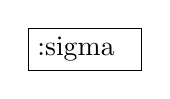
\begin{tikzpicture}
\node[draw,text width=1.2cm] at (2,-2) {\code{:sigma}};
\end{tikzpicture}
\end{lrbox}

\newsavebox\boxsempty
\begin{lrbox}{\boxsempty}
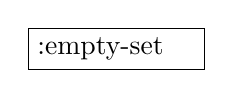
\begin{tikzpicture}
\node[draw,text width=2.0cm] at (2,-2) {\code{:empty-set}};
\end{tikzpicture}
\end{lrbox}


\begin{frame}{Rewrite: $1\to 2\to 3\to 4\to\colorbox{orange!30}{\Huge 5}\to 6\to 7\to 8\to 9$}
  \begin{tabular}{ll}
    Replace \usebox\boxstop~with \code{\textcolor{greeny}{then}} branch. &
    Replace \usebox\boxsempty~with \code{\textcolor{red}{else}} branch.
  \end{tabular}

  \only<1>{\centerline{\includegraphics[height=0.8\textheight]{ldd-4.pdf}}}%
  \only<2>{\centerline{\includegraphics[height=0.8\textheight]{ldd-5.pdf}}}
  
\end{frame}


\begin{frame}{Rewrite: $1\to 2\to 3\to 4\to 5\to \colorbox{orange!30}{\Huge 6}\to 7\to 8\to 9$}
  Duplicate tree, and introduce \colorbox{pink!30}{\code{if (typep x I) \code{\textcolor{greeny}{then}} ... \code{\textcolor{red}{else}} ...}}

  \begin{columns}
    \begin{column}{0.5\textwidth}
      \includegraphics[height=0.8\textheight]{ldd-5.pdf}%
    \end{column}

    \begin{column}{0.5\textwidth}  %%
      \includegraphics[height=0.8\textheight]{ldd-6.pdf}%
    \end{column}    
  \end{columns}
\end{frame}

\begin{frame}{Rewrite: $1\to 2\to 3\to 4\to 5\to \colorbox{orange!30}{\Huge 6}\to 7\to 8\to 9$}
  Duplicate tree, and introduce \colorbox{pink!30}{\code{if (typep x I) \code{\textcolor{greeny}{then}} ... \code{\textcolor{red}{else}} ...}}

  \centerline{\includegraphics[height=0.8\textheight]{ldd-6.pdf}}  %
\end{frame}


\begin{frame}{Rewrite: $1\to 2\to 3\to 4\to 5\to 6\to \colorbox{orange!30}{\Huge 7}\to 8\to 9$}
  \begin{tabular}{ll}
  In \code{\textcolor{greeny}{then}}: \colorbox{pink!30}{Supertypes of \code{I} $\to$ \code{:sigma}}.&
  In \code{\textcolor{red}{else}}: \colorbox{pink!30}{Subtypes of \code{I} $\to$ \code{:empty-set}}.
  \end{tabular}

  \only<1>{\centerline{\includegraphics[height=0.8\textheight]{ldd-6.pdf}}}%
  \only<2>{\centerline{\includegraphics[height=0.8\textheight]{ldd-7.pdf}}}
\end{frame}


\begin{frame}{Rewrite: $1\to 2\to 3\to 4\to 5\to 6\to 7\to \colorbox{orange!30}{\Huge 8}\to 9$}
  \begin{tabular}{ll}
      \colorbox{pink!30}{\code{(not :sigma)} $\to$ \code{:empty-set}} &    
      \colorbox{pink!30}{\code{(not :empty-set)} $\to$ \code{:sigma}}
  \end{tabular}

  \only<1>{\centerline{\includegraphics[height=0.8\textheight]{ldd-7.pdf}}}%
  \only<2>{\centerline{\includegraphics[height=0.8\textheight]{ldd-8.pdf}}}
\end{frame}

\begin{frame}{Rewrite: $1\to 2\to 3\to 4\to 5\to 6\to 7\to 8\to \colorbox{orange!30}{\Huge 9}$}
  \begin{tabular}{ll}
    Replace \usebox\boxstop~ with \code{\textcolor{greeny}{then}} branch. &
    Replace \usebox\boxsempty~ with \code{\textcolor{red}{else}} branch.
  \end{tabular}

  \only<1>{\centerline{\includegraphics[height=0.8\textheight]{ldd-8.pdf}}}%
  \only<2>{\centerline{\includegraphics[height=0.8\textheight]{ldd-9.pdf}}}
  

\end{frame}


\begin{frame}{Rewrite: Summary}
  Code has been rewritten so that \Emph{any type check occurs no more than once}.

  \begin{columns}
    \begin{column}{0.5\textwidth}
      \usebox\typecaseAbox
    \end{column}
    \begin{column}{0.5\textwidth}  %%
      \usebox\typecaseKbox
    \end{column}
  \end{columns}

  And it is clear the code never returns \code{nil}.

\end{frame}





